%# -*- coding: utf-8-unix -*-
% !TEX program = xelatex
% !TEX root = ../thesis.tex
% !TEX encoding = UTF-8 Unicode
%%==================================================
%% chapter01.tex for SJTU Master Thesis
%%==================================================

%\bibliographystyle{sjtu2}%[此处用于每章都生产参考文献]
\chapter{绪论}
\label{chap:intro}
\section{研究背景与意义}
本论文由上海市发展和改革委员战略新兴产业专项项目“基于物联网的当代艺术品电子商务公
共服务平台”、上海市经济和信息化委员会、上海市人力资源和社会保障局项目“上海市物联网技术
高技能人才培养基地RFID 应用实训设施设备环境资助”两个课题支撑。

\begin{figure}[!htp]
  \centering
  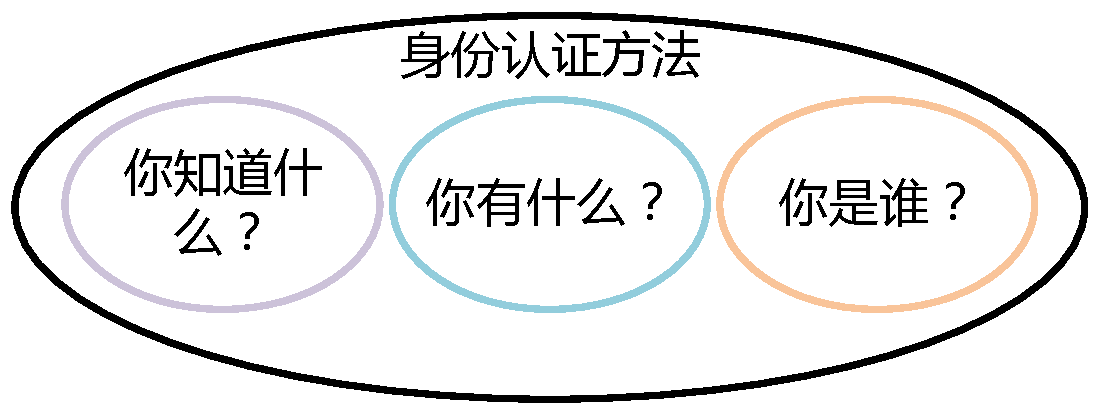
\includegraphics[width=0.7\textwidth]{figure/identification-method.pdf}
  \bicaption
    {身份认证方式}
    {Identification methods}
  \label{fig:identification-method}
\end{figure}
随着信息技术的兴起和广泛应用,许多应用需要用户首先进行登录操作,这其实就是身份识别方式,只有通过了通过身份认证的用户才会被系统认为是授权用户,用户才能访问到自己的隐私数据,比如地址信息、财务信息等。如图~\ref{fig:identification-method}所示,用户的身份方式可以为分为三种~\cite{Huang2011A}:
\begin{enumerate}[label=(\arabic*)]
    \item \textbf{根据用户知道的信息来证明身份。(你知道什么?)}日常生活中,我们以前最常用的是密码登录,这是一种依赖用户知道什么来识别是否为授权用户,但用户知道的密码被泄露,恶意用户输入相同的密码也会被系统识别为授权用户。
    \item \textbf{根据用户拥有的东西来证明身份。(你有什么?)}我们回家会使用钥匙开门,钥匙就是我们所拥有的东西,比起用户知道的信息,此处则体现为用户拥有的物理实体。
    \item \textbf{根据用户独一无二的身体特征证明身份。(你是谁?)} 随着智能手机的技术进步和普及,依靠智能手机上丰富的传感器配置,用户的认证方式也变多多样话起来,目前人脸和指纹识别已经被用于手机系统登录和移动支付。人脸~\cite{12717}、指纹~\cite{Andrew2005Handbook}、虹膜~\cite{Wildes1997Iris}等是人体上的固有特征,在随着时间变化上呈稳定状态,这样的认证方式比密码认证更加安全。 除此之外,个人独特的行为特征也可以被用于身份认证,比如:语音识别~\cite{Rashid2008Security}、唇语识别~\cite{Cetingul2006Discriminative}、步态识别~\cite{Boulgouris2005Gait}、手写签名识别~\cite{Plamondona1989Automatic}等。 
\end{enumerate}

手写签名作为个体的一种重要的行为特征,在金融、法律、政府等领域得到广泛应用,用于用户身份的识别,来识别一份文件的真实性。 相对应得,这种认证方式也会收到恶意用户的攻击,举个例子,攻击者可以仿造存款用户的签名去一张取款支票上签名从而去银行取款,会造成实际用户的财产损失,降低银行存款安全性,大则可引发金融灾难。 而在政府或军事领域,仿造签名会造成更加难以想象的结果,造成社会不公平和混乱。 因此,在这些签名进行授权的领域,签名的识别变得尤其重要。在很久以前甚至现在,签名的识别靠人工进行,签名验证者用户的历史签名在判断当前的签名是否为真实签名。这种方式,需要耗费昂贵的人力资源,且依赖于签名认证员的个人能力,容易造成错误。

信息技术将签名认证方式进行了自动化,自动签名认证系统得到研究和应用。 自动签名认证系统根据捕捉签名的方式不同,可以被分为两大类:离线签名认证系统和在线签名认证系统。 离线签名认证系统依靠签名图像的静态数据进行签名的比较来识别,而在线签名认证系统则依靠用户书写过程中记录下的时间序列数据(如书写速度、笔的压力等)来进行比较和识别。由于,外加的时间维度信息,通常在线签名认证系统的表现由于离线签名认证系统。

\begin{figure}[!htp]
  \centering
  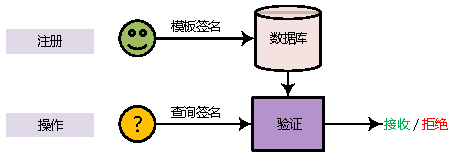
\includegraphics[width=0.7\textwidth]{figure/verification-work-flow.pdf}
  \bicaption
    {签名认证过程}
    {Signature verification architecture}
  \label{fig:signature-verification-architecture}
\end{figure}

无论是人工的签名识别还是自动签名认证系统,签名的识别的过程都符合图~\ref{fig:signature-verification-architecture}所示的这个签名认证过程。 在注册过程,用户需要收入多个他/她的签名给系统存入数据库作为模板签名;在操作过程,用户签下签名作为查询签名提交给系统,系统将这个查询签名和模板签名进行比较,判断查询签名是否为真实签名。

一个签名认证系统,识别任务的关键问题在于二方面:
\begin{enumerate*}[label=\itshape\alph*)\upshape]
    \item 需要能精准跟踪手写签名过程的行为信息。由于手写签名过程,笔记变化多样,而且运动幅度较小,对传感器的敏感度有较高要求。
    \item 用户体验和判别精度。用户体验体现在设备对用户的影响,比如是否需要特殊设备、是否需要用户佩戴设备等,还体现在模板签名数量。用户体验可能会和判别精度发生冲突,比如减少的模板签名数量会导致判别精度下降,复杂的设备则能更细粒度跟踪签名运动轨迹,有利于判别精度的提升。
\end{enumerate*}

开展自动手写签名认证的研究才能顺应用户对用户体验和财产安全提升上的诉求,将一部分人力资源从签名识别中解放出来,提高签名识别的准确率和稳定性,有利于维护金融和社会稳定。探索签名的捕捉方式,可以降低签名认证的成本,让签名认证系统在用户中快速普及。 目前国内外对手写签名认证的研究有很多基于开放数据集进行研究,存在一些问题,在普适性和用户体验上有待提高,所以本课题具有较好的研究意义和指导价值。

\section{国内外研究的现状}
如上文所述,手写签名认证研究的关键问题主要在两个方面,一是数据的来源问题,而是手写签名认证的建模问题。下面本节将从这两个方面对现有研究进行介绍。

(1) 数据来源问题的研究现状

在数据来源方面,现有的手写签名认证系统的研究主要依赖于惯性传感器、手写平板设备和扫描图像。其中前二者可用于实现在线签名认证系统,而离线签名认证系统则依赖于扫描图像的数据来源。

基于惯性传感器的方法~\cite{levy2018handwritten,griswold2019wearables,bunke2011online}利用穿戴在手上的惯性传感器 (速度计、陀螺仪等) 跟踪手部运动,提取个人签名时独特手部运动特征。这种方法,要求用户的穿戴的设备会给用户造成额外的困扰,设备穿戴的位置不宜固定,且会对结果造成较大影响。这里的惯性传感器设备包括:定制设备、腕表和装有惯性传感器的笔。

基于手写平板设备的方法~\cite{fischer2015robust,kholmatov2005identity,sae2013simple}利用手写笔或者手指在平板书写留下的动态轨迹来识别签名。这样的轨迹在静态轨迹基础上,还能获得书写时对平板压力和轨迹变化速度等时间序列,相比单单用静态图像可以大大提高判别精度。但是这样的设备需要一个手写平板,虽然我们可以利用上智能手机代替,但是这种方式限制了字迹不能写在平板上,而不能写在纸上这样我们生活最常见的场景。

基于扫描图像的方法~\cite{hafemann2017learning,hafemann2018fixed,ferrer2005offline,kalera2004offline}使用扫描仪扫描并切割出的签名图像,这种直接比较静态图像,与人工判别的方式在数据来源上有相似之处。由于没有写的过程,这种只比较写出结果的方法,无法判断出在字迹上看起来很相似仿造签名,尽管仿造者用较多的时间才仿造出了这个签名。但这种签名认证方式很有通用性和较好的用户体验,不会给用户签名过程造成干扰,用户可以依照平时的签名习惯来签名。

(2) 手写签名认证建模问题的研究现状

在手写签名认证建模方面,方法有多种多种,首先针对离线和在线签名认证系统需要采取不同的建模方法。在离线签名认证系统中,则能采用图像匹配的方法,比如人工神经网络(Artificial Neural Network, ANN)~\cite{chandra2016offline}、像素匹配 (Pixel Matching Technique, PMT)~\cite{bhattacharya2013offline}等。 在在线签名认证系统中,又可以分为两种:\textit{a)} 基于函数的方法,使用长短时记忆网络 (Long Short-Term Memory, LSTM)~\cite{hochreiter1997long}, 隐马尔科夫模型 (Hidden Markov Model, HMM)~\cite{rabiner1986introduction}, 动态时间规整 (Dynamic Time Warping, DTW)等这些函数型方法直接在时间序列上进行处理并识别;\textit{b)} 基于特征的方法,这种方法首先对时间序列从时域数据转化为频域数据,可以用到的变换方法有离散傅里叶变换 (Discrete Fourier Transform, DFT)、离散余弦变换 (Discrete Cosine Transform, DCT)~\cite{}等,在频域特征上进行特征选择从而实现数据的降维,在利用提取到的特征进行比较或者分类。匹配方法也可以使用DTW或者欧式距离,而分类方法可以使用一些机器学习方法~\cite{周志华2016机器学习},比如支持向量机 (Support Vector Machine, SVM)、随机森林 (Random Forest)、朴素贝叶斯 (Naive Bayes)等。这些很多方法都是在公开数据集上进行实现和评估的,当有新数据源时,我们需要设计新的合适的模型。而且,由于使用的是公开数据集,这些研究很少评估系统的鲁棒性,比如不同时间段对签名的影响。

\section{本文研究内容与创新点}
\subsection{研究内容与所做的工作}
在本文中,我们针对现有存在的主要问题着重研究设计一种非侵入式、鲁棒的、安全的、低延迟的在线手写签名认证方案,主要的研究内容和本文主要所做的工作如下:

(1) 手写签名认证数据源的研究

本文提出利用声波感知技术来跟踪手写签名时的运动手部和笔的运动状态,进而推断是否为本人签名。声波对我们来说不是陌生的信号,我们用声带发射声波,用耳膜接收声波,以此来实现对这个世界的感知。普通的智能手机上的扬声器和麦克风便能发射和接收声波,近年来,声波感知研究大量涌现,比如轨迹追踪~\cite{wang2016device,mao2016cat,yun2017strata}、呼吸检测~\cite{WangContactless,wang2018c}、手势识别\cite{ruan2016audiogest,gupta2012soundwave,aumi2013doplink,ling2018ultragesture}、成像\cite{mao2017aim}等。
假设声波信号的频率和传播速度分别是17000 Hz 和 346 m/s, 那么波长经计算为  $346/17000\approx0.02m$. 这么小的波长意味着声波的相位信息对周围物体的运动很敏感。本文采用声波的相关信息,利用计算弦的方法避开了求相位时去直流的问题,实现了微小动作的跟踪。


(2) 手写签名认证模型的研究

所有手写签名认证系统的大致框架前文已经有所提及,本文则针对声波的相位相关信息设计了合适的特征提取和用户独立的识别模型。手写签名动作所产生的影响在相位信号中体现为低频信号,而高频信号则是由环境或者硬件造成的噪声所产生。因此可以通过将时域数据转换到频域数据,然后提取低频系数的方法,将手写签名动作的信息提取出来。DFT是一种常见的获取频域数据的方法,但它的系数是2倍冗余的复数系数,所以我们采用DCT作为到频域数据的转换方法,并提取其前几个低频系数作为特征。当判别一个查询签名是否为真的时候,需要获取查询签名与模板签名之间的相似度,在此处,便是比较查询签名的特征与模板签名特征的之间的相似度。本文对多个模板签名的特征进行融合操作,获得几个固定数目的特征矩阵,查询签名的特征矩阵和这些矩阵作差获得相似矩阵。最后设计比传统分类器有更好表现的深度神经网络 (Deep Neural Network, DNN)\cite{Schmidhuber2015Deep} 作为一个二分类器,去分类相似矩阵。

(3) 基于声波的手写签名认证的系统实现和性能评估分析

本文针对所提出的基于声波的手写签名认证的方案,利用三星Galaxy S6智能手机设计并实现基于声波的手写签名认证系统,并且对其进行了全面的评估,包括准确性的度量、鲁棒性测试、安全性测试、微基准测试、性能测试等。准确性测试以 AUC (Area Under Curve) 和 EER (Equal Error Rate) 作为度量指标。在鲁棒性测试中,改变环境、距离、日期来对系统进行测试,观察准确性的变化。在安全性测试中,是模拟重放攻击,从而测试系统对此类攻击的抵抗能力。在微基准测试中,改变一些超参数,来观察系统的变化,以便设置较合适的超参数。在性能测试中,度量系统延迟,来判断系统是否具有良好的用户体验和是否对硬件要求过高。


\subsection{研究创新点}

本文主要有如下两个方面的创新点:
\begin{enumerate}[label=(\arabic*)]
    \item 本文第一次提出使用声波感知技术来实现一个在线签名认证系统,并基于一个三星Galaxy S6智能手机实现了一个非侵入式、用户友好、安全、低延迟、准确的在线签名认证系统。而且相比于之前的声波感知技术,在避免去直流的前提下,提取到了相位相关信息,用以跟踪手写签名时所产生的微小的动作。

    \item 本文针对新产生的信号,设计了特征提取方法和分类方法,并在进行了高效地实现。使用DCT提取信号中低频的有用的部分作为手写签名行为的特征,并使用深度学习进行分类,相比传统的分类方法获得了更好的表现。本文利用三星Galaxy S6智能手机设计并实现了基于声波的在线签名认证系统,全面评估了系统的性能。实验结果表明,本文提出的基于声波的在线签名认证系统的AUC可以达到98.7\%, EER可以达到5.5\%,并且是个安全、高效、鲁棒、低延迟的系统。
\end{enumerate}

\section{本文结构}

本文共分五章,每章的内容安排如下:

第一章为绪论,主要阐述了手写签名认证研究的背景意义、国内外相关技术的发展现状、本文的研究内容以及主要的创新之处。

第二章是手写签名认证相关技术的分析,首先分别从手写签名认证中的感知技术和手写签名认证中的建模方法两个方面对现有的研究进行了综述,然后分析总结了现有研究存在的问题。基于存在的问题,提出了本文的技术路线,最后介绍了本文中所涉及到的相关理论和技术。

第三章是基于声波的手写签名认证的关键技术研究,首先对要解决的问题进行了描述,然后提出一种基于声波的手写签名认证方案,该方案主要包含四个模块,对应了四种关键技术,然后依次对涉及到的声波相位相关信号感知技术、特征提取技术、相似性度量技术和深度学习模型进行了研究,详细描述了方案中各模块的设计思想和技术细节。

第四章首先对基于声波的手写签名认证方案进行了实验验证以及分析,手写描述了实验方法和采集的数据集,提出验证指标和用于对比的方案,之后实验验证本文方案的识别性能,最后探究影响识别性能的主要因素。

第五章基于本研究提出的基于声波的手写签名认证方案实现了一个基于安卓智能手机的手写签名认证系统,首先是对系统的用户需求进行分析,然后基于分析完成系统架构的设计,最后进行一系列评估实验来评估系统的性能效果。第六章是总结和展望,对本文的研究内容进行了总结,同时针对本文存在的不足,对未来的工作进行了一定的展望,并提出了系统可以改进的关键点。

\chapter{手写签名认证相关技术分析}
\label{chap:related-work}
目前手写签名认证的任务呈现普适性、便利性、模型用户无关的发展趋势,对实施技术的要求越来越高,在本章中我们将首先介绍手写签名认证研究综述,分析总结现有的研究存在的问题,然后针对存在的问题提出本文的技术路线,最后对本文涉及到的相关理论与技术进行介绍。
\section{手写签名认证研究综述}
手写签名认证研究所涉及到的技术领域比较广泛,如传感器技术、图像技术、通信技术、机器学习等等。应用这些技术需要解决的最核心的问题主要是两点,即“签名行为的数据怎么采集”和“采集到的数据怎么处理”。所以在手写签名认证的研究综述中,本文分别从手写签名认证中的感知技术和手写签名认证中的建模方法两方面进行综述。
\subsection{手写签名认证中的感知技术}
(1) 基于惯性传感器的手写签名认证
  
在手写签名的过程中,签名者通过手和笔的运动来留下签名字迹,运动过程中,手和笔的运动加速度和方向会发生变化,因此可以通过给手或者笔配备惯性传感器来实现对此运动过程的记录。常见的惯性传感器包括加速度计和陀螺仪,这两个惯性传感器均可产生三维的时间序列数据,分别记录物体线加速度和角运动,用于描述物体在三位空间中的运动状态。装配方式有两种:将惯性传感器装在手上,如智能腕表;将惯性传感器装在笔上。

\begin{figure}
  \centering
  \begin{minipage}[t]{0.3\textwidth}
    \centering
    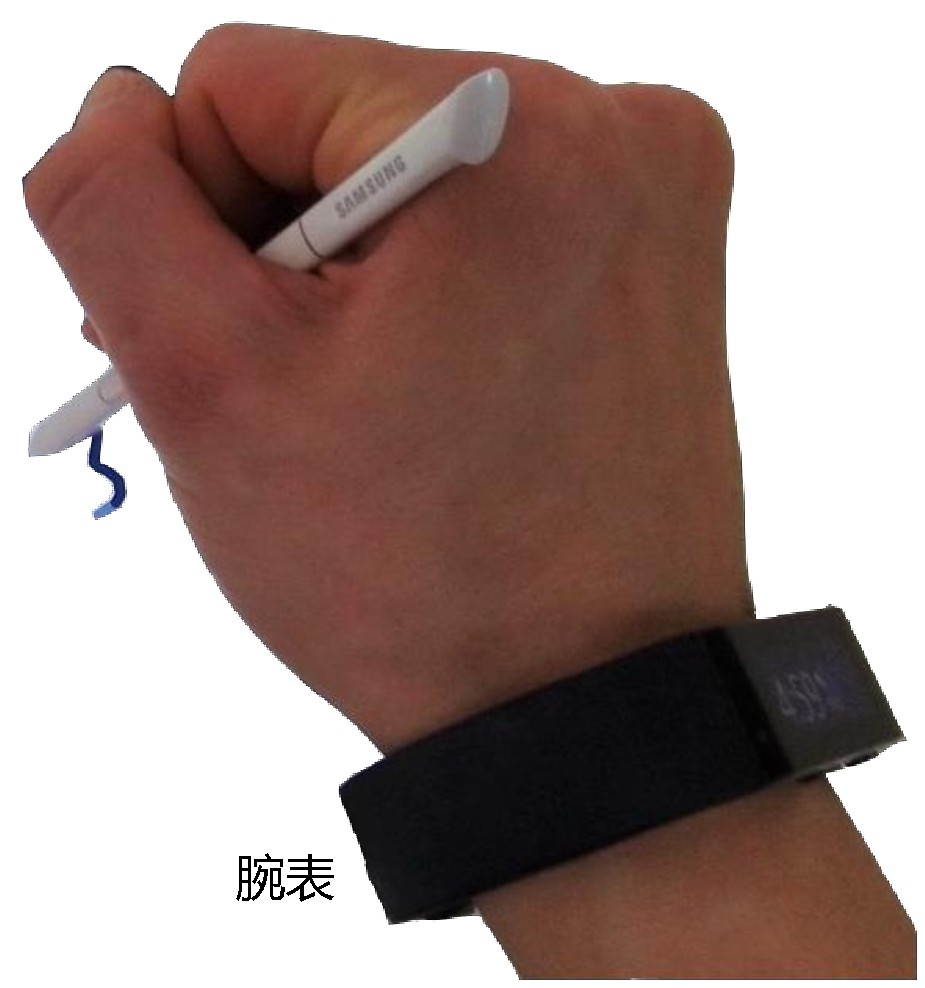
\includegraphics[width=\textwidth]{figure/smartwatch.pdf}
      \bicaption{用腕表上惯性传感器}
      {Using inertial sensors on swatches}
        \label{fig:smartwatch-inertial-sensor}
  \end{minipage}
  \centering
  \begin{minipage}[t]{0.49\textwidth}
    \centering
    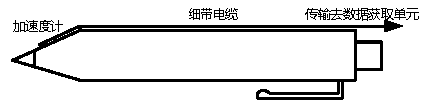
\includegraphics[width=\textwidth]{figure/acceleration-pen.pdf}
    \bicaption
    {用笔上的惯性传感器}
    {Using inertial sensors on pens}
    \label{fig:pen-inertial-sensor}
   \end{minipage}
\end{figure}
如图~\ref{fig:smartwatch-inertial-sensor}所示,基于腕表,Alona~\cite{Levy2018Handwritten}等人提出一种可穿戴的手写签名认证系统,它使用一个戴在签名手上的智能腕表上的惯性传感器和加速度计实现对签名动作的记录,虽然腕表目前的普及率还选不如智能手机,但腕表仍在受到大众的欢迎,所以这种方法具有普适性。Isaac\cite{8698222}等人使用腕表是实现了在多个场景下的手写身份识别,并对多种不同强度的攻击方式进行评估。使用如图~\ref{fig:pen-inertial-sensor}所示,基于笔上的加速度计,Bunke~\cite{Bunke2015Online}等人在普通笔的笔尖附近贴上了一个带线的加速度计,通过细带电缆将加速度时间序列传输到电脑端,依此分析签名动作。

(2) 基于扫描图像的的手写签名认证
\begin{table}[!hpb]
  \centering
  \bicaption
    {真实签名与仿造签名图像}
    {Genuine and forged signatures}
  \label{tab:signatures-images}
  \begin{tabular}{|c|m{0.2\textwidth}|m{0.2\textwidth}|m{0.2\textwidth}|} \toprule 
    类型 & 真实签名 & 熟练仿造签名 & 不熟练仿造签名\\ \midrule
   简单& 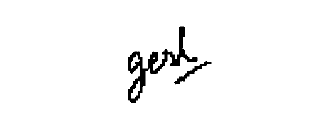
\includegraphics[width=0.2\textwidth]{figure/signature-1.png}&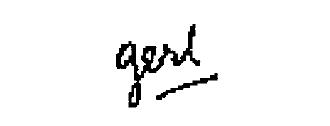
\includegraphics[width=0.2\textwidth]{figure/signature-2.png}&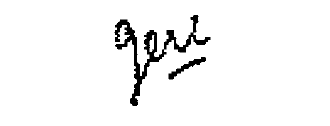
\includegraphics[width=0.2\textwidth]{figure/signature-3.png} \\ \midrule
    草书&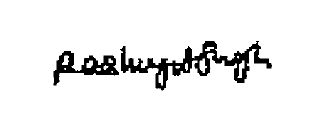
\includegraphics[width=0.2\textwidth]{figure/signature-4.png}&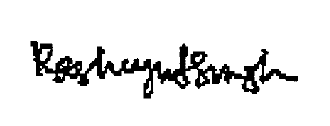
\includegraphics[width=0.2\textwidth]{figure/signature-5.png}&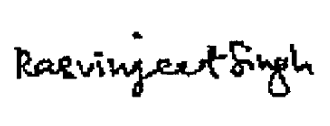
\includegraphics[width=0.2\textwidth]{figure/signature-6.png} \\ \midrule
    图形&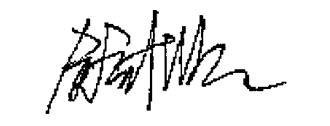
\includegraphics[width=0.2\textwidth]{figure/signature-7.png}&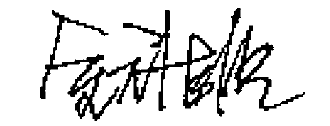
\includegraphics[width=0.2\textwidth]{figure/signature-8.png}&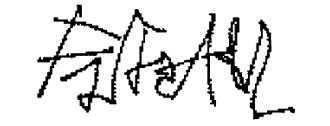
\includegraphics[width=0.2\textwidth]{figure/signature-9.png} \\ 
        \bottomrule
  \end{tabular}
\end{table}

如图~\ref{tab:signatures-images}所示,在图像上,签名通常可以被分为三类~\cite{Hanmandlu2005Off}:简单的、草书的、图形的签名。简单的签名便是平时的普通签名;草书签名是写的过程有比划连在一起的签名;图形的签名则是用草书方式描述几何模式的签名。从图像上真实签名、熟练仿造签名、不熟练仿造签名之间有很大相似之处,但是细看不同之处也有很多。离线签名认证利用这些从纸上扫描出来的图像进行识别。

Madasu~\cite{Hanmandlu2005Off}等让签名者使用黑笔在白纸上签名,之后使用扫描仪以200 dpi的分辨率扫描获得图像,并经过50\%的重采样将像素点数量减少到原来的一半。40个志愿参与数据集构建,每个志愿者提供15个真实签名和15个仿造签名,总共2400个签名图像。Subhash~\cite{chandra2016offline}等人邀请了18个志愿者,每个志愿者提供15个真实签名和15个仿造签名,总共540个尺寸为$850\times360px$的签名图像。除了自己手机签名数据集外,目前公开的签名图像数据集有:MCYT\footnote{http://atvs.ii.uam.es/atvs/mcyt75so.html}、CEDAR\footnote{https://cedar.buffalo.edu/Databases/CDROM1/}、Brazilian PUC-PR~\cite{freitas2008brazilian}. 签名的公开数据库文字上以英文居多,Brazilian PUC-PR则提供巴西葡萄牙语的签名数据。采集签名的方式,最传统的可以直接让志愿者写在纸上,然后扫描,这种方式较为费力。而最近,可以让签名者将签名写在平板上,仅仅使用静态轨迹数据就可以作为离线签名的数据集,同时兼顾离线签名认证研究和在线签名认证研究对数据集的需求。

(3) 基于手写平板设备的手写签名认证

\begin{figure}[!htp]
  \centering
  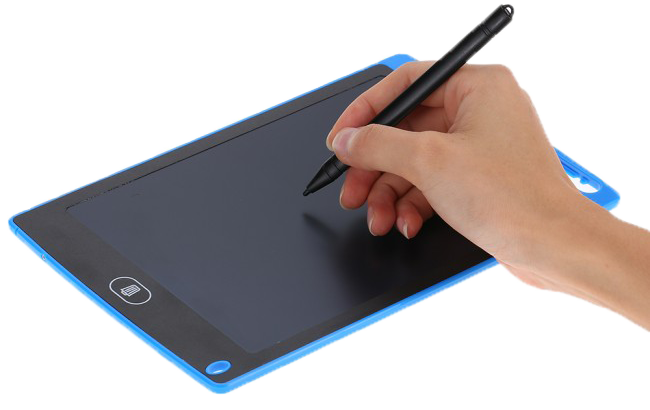
\includegraphics[width=0.5\textwidth]{figure/tablet.png}
  \bicaption
    {在平板上签名}
    {Signing on a tablet}
  \label{fig:signing-tablet}
\end{figure}
如图~\ref{fig:signing-tablet}所示,签名使用使用手写笔在平板上签名,由平板记录签名轨迹,手写屏除了记录轨迹还能记录压力值,如果使用智能笔则还能记录笔的倾斜角,因此时间序列数据可以包括:采样点的二位坐标、笔尖压力值、笔的水平偏角和垂直偏角。Alona~\cite{Levy2018Handwritten}等人在用腕表上惯性传感器跟踪签名动作时候,同时用手写记录签名轨迹,将平板上轨迹数据除了可以提给仿造者提供仿造学习材料,还可以用于和两个经典系统~\cite{fischer2015robust,kholmatov2005identity}做对比实验。目前,可用于在线签名认证研究的公开数据集有:MCYT-100\footnote{http://atvs.ii.uam.es/atvs/mcyt100s.html}、SUSIG~\cite{kholmatov2006sigsa}、SVC2004~\cite{10.1007/978-3-540-25948-0_3}、SCUT-MMSIG~\cite{10.1007/978-3-319-69923-3_78}等。

MCYT-100是MCYT数据库的一个子集,包含100个签名者的数据,每个签名者有25个真实签名和25个仿造签名,总共5000个签名样本。至于SUSIG数据库,Kholmatov~\cite{kholmatov2006sigsa}等人使用一个分辨率为300 dpi、具有128层垂直压力感知、100 Hz采样率的压力感知触摸平板,邀请110位志愿者参与真实签名的收集,其中包括年龄在21岁到52岁之间的29位女性和81位男性,每个位志愿者分两个时间段提供20个真实签名,而仿造签名由仿造者观看签名过程并联系后为每个真实签名者提供5个仿造签名,他们同时用实验结果签名是一个复杂度取决于签名者的生物特征。SV2004是2004年香港科技大学举办在线认证比赛提供的数据库,针对比赛中的两个任务,该数据库提供两个数据集,每个数据集都包含100个签名集合,每个签名集合包含20真实签名和20熟练仿造签名,不同是其中一个数据集只包含坐标时间序列,而另外数据集则还包含笔的方向和压力,两个数据集前40个集合完全不同,而后60个集合仅仅是笔的方向和压力不同。比赛中,成绩最好的第一个任务EER=2.84\%,第二个任务EER=2.89\%。SVC2004包含中文签名和英文签名,SCUT-MMSIG则是由华南理工大学采集的纯中文签名,所以如果做针对中文签名认证研究的研究者可以考虑这两个签名数据作为评估数据集。

此领域的研究者基于公开数据集做了很多工作。算法~\cite{kholmatov2005identity}提出SVC2004是的冠军提出。2015年提出的一个算法~\cite{fischer2015robust}在两个数据集上进行了评估,在MCYT数据集上使用5个模板签名时在随机仿造(random forger)和熟练仿造(skilled forger)情况下的EER分别为1.06\%和3.94\%,在SUSIG数据集使用5个模板签名时在随机仿造和熟练仿造情况下的EER分别为1.34\%和3.09\%。

\subsection{手写签名认证中的建模方法}

已经有很多文章对签名认证研究进行了综叙,如80年代的Rejean~\cite{plamondon1989automatic}等人的综叙,那时研究者开始用人工神经网络实现签名认证,还,有90年代的Franck~\cite{leclerc1994automatic}和2000年代的Donato等人~\cite{impedovo2008automatic}的综述,在2012年Donate等人对之前的综述进行了补充~\cite{impedovo2012handwritten}。近期,Luiz G.~\cite{hafemann2017offline}等人对离线签名认证进行了综述,并加入基于深度学习的相关研究内容。Prathiba~\cite{prathiba2014online}等人对在线签名认证进行了综述。

Kai~\cite{huang1997off}等人提取了签名图像的多种粒度的局部对比的几何特征,为每个力度的特征使用一个适配的多层感知机,多个感知机的输出作为一个决策感知机的输入,决策感知机用于输出最后二分类的结果,在一个超过3000个样本的数据库中达到90\%的分类准确率。为所有用户而训练的模型称为写者独立模型(writer-independent model, WI model),而需要为每个用户训练一个的模型称为写着依赖模型(writer-dependent model, WD model)。有些系统会使用熟练仿造签名进行用户独立模型的训练~\cite{rivard2013multi,eskander2013hybrid},而有些系统使用熟练仿造签名进行用户独立模型训练~\cite{yilmaz2016score,rantzsch2016signature,hafemann2017learning},再用另外一个分开的数据集进行测试。有些系统混合使用用户独立模型和用户依赖模型,使用用户独立模型用于特征提取,利用提取到的特征为每个用户训练一个小型的用户依赖模型,综合了两种模型的优点。随着深度学习在图像领域的广泛应用,现在可以用DNN直接从图像中学习得到特征。Hafemann~\cite{hafemann2016writer}等人使用一个卷积神经网络(Convolutional Neural Network, CNN)作为特征提取器,在用SVM为每个用户训练一个用户依赖模型,之后进步提出了多任务的卷积神经网络框架~\cite{hafemann2017learning},可同时提取到区分签名真实性和用户间差异的特征。

来自签名的动态特征提供提供了某个时间的比划数目和顺序,速度,笔的压力等相关信息,可以提高签名变得更加具有唯一性。 Alisher~\cite{kholmatov2005identity}等人的在线签名认证系统将签名的识别视为一个二分类的模式识别问题。DTW被用于建立给定签名的合法性:给定一个签名与被申明用户的参考签名计算DTW距离,计算出与最近、最远、模板参考签名的DTW距离,生成3维的特征向量用于后续的分类。在使用熟练仿造者的测试用,EER达到2.8\%。S.A. Daramolo~\cite{daramola2010efficient}等人为了建立签名的特征序列之间的一致关系,DTW被用于训练和分类。Alona~\cite{levy2018handwritten}等人结合使用DCT和DTW,得到一个特征向量,最后输入到一个用户独立的二分类进行判别。HMM被证明可以有效用于签名认证,应为它可以高度适应个体间差异。Mohammad M. Shafli 和 Hamid R. Rabiee~\cite{shafiei2003new}介绍了使用变长分段和HMM实现的在线签名认证系统,实现了错误接受率(False Accept Rate, FAR)和错误拒绝率(False Reject Rate)分别为4\%和12\%的性能。Syed Khaleel Ahmed~\cite{ahmed2009automatic}等人设计的签名认证系统由4个模块组成,分别是特征提取模块、参考模块、样本模块、智能决策模块。特征提取模块用于捕捉二位坐标和笔的压力的时间序列。参考模块用于存储训练数据。样本模块包含用于验证的数据。智能决策模块则是一个自组织映射神经网络,用于对数据进行聚类,将高维数据映射为1或2维数据。%Alona~\cite{levy2018handwritten}等人使用DCT对惯性传感器的数据转换去前几位低频系数,减少了数据量,将查询签名的DCT系数和模板签名的低频系数求DTW距离并去最小值,得到一个特征向量,最后输入到一个用户独立的二分类进行判别。

\section{现有研究存在的问题}
根据上文对于手写签名认证的研究综述,现分别从手写签名认证中的感知技术和建模技术这两方面对现有研究存在的问题进行分析总结。

(1) 手写签名认证的感知技术中存在的问题

目前,通常采用的手写签名认证中的感知技术方案主要有三种——基于惯性传感器、基于扫描图像、基于手写平板设备的解决方案。其中,基于惯性传感器的主要问题是,需要用户或者笔上佩戴惯性传感器,会给用户带来不便利性:如果是笔上安装惯性传感器,则要求定制的笔,不便于推广;如果是要求用户佩戴腕表之类的设备,则该设备必须在用户写字的手上,在可穿戴设备还没大量普及的前提下该要求过于苛刻,而且腕表在手上的位置变化也会提高判别的错误率。基于扫描图像的方法,比较符合用户的习惯,但是由于动态特征的缺失,熟练的仿造者可以话足够的时间去仿造他们的签名已达到在静态形状上尽可能像,这给离线签名认证系统带来了巨大的挑战。基于手写平板设备的方法,需要一个可以手写平板,如果用手指写则不符合用户平时的签名习惯,如果也是用笔在平板上写并且给予书写轨迹的反馈,还是需要特殊的设备,提高了普及化的难度。

(2) 手写签名认证的建模技术中存在的问题

DTW是一种非常经典用于计算两个不同长度的序列距离的算法,其在模式识别中的应用十分广泛。然而,DTW技术具有两个明显的缺点:(1)计算开销大,需要更多时间;(2)对仿造签名进行规整使得验证更加困难。而且HMM模型是无记忆性的,它的当前状态只与其前一个状态有关,无法利用更多复杂信息。使用深度学习进行用户无关的模型训练会引发巨大的训练开销,而且越是复杂的网络要求有足够大的数据集防止其过拟合。目前的系统大多在公开数据集进行测试,过于追求精度的提升,很少有度量在识别时间上的开销,因此复杂的方法在时间中不一定可行。

\section{本文的技术路线}
\begin{figure}[!htp]
  \centering
  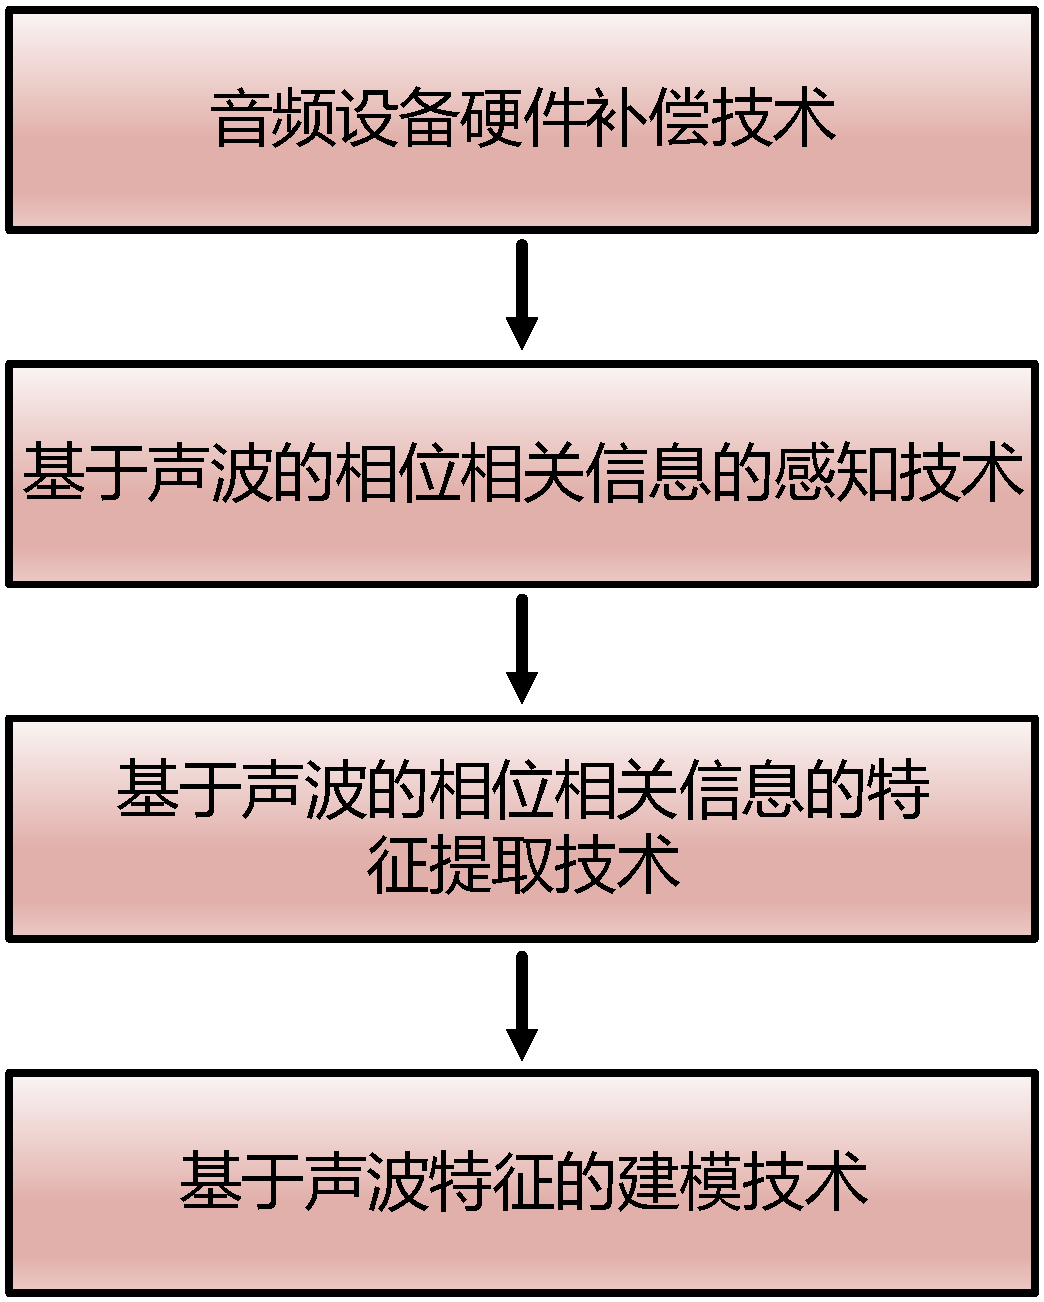
\includegraphics[width=0.4\textwidth]{figure/technique-road.pdf}
  \bicaption
    {本文的技术路线}
    {The technology roadmap}
  \label{fig:technology-roadmap}
\end{figure}
本文通过深入分析现有研究,针对目前手写签名认证中的感知技术和手写签名认证中的建模方法的研究中存在的问题,提出了本文的技术路线。技术路线如图~\ref{fig:technology-roadmap}所示,其中主要分为具有递进关系的四种技术研究,分别是音频设备硬件补偿技术、基于声波的相位相关信息的感知技术、基于声波的相位相关信息的特征提取技术、基于声波特征的建模技术。其中的箭头表示了这几种技术步骤之间的依赖关系,下面将分别介绍这四种技术。

(1) 音频设备硬件补偿技术

本文的数据采集和原型系统实现基于智能手机上的音频设备。然而,智能手机上的音频设备主要用于娱乐、通信、降噪等,其主要设计用途并不包括声波感知,因此当时利用智能手机发送高频的声波信号(17 kHz以上),尤其是同时发送多个高频声波信号时,每个频率说声波实际发送能量差异可能会很大。本文针对智能手机上的音频设备的硬件不足,进行了硬件补偿,以便目标频率声波的发射能量不至于太小。

(2) 基于声波的相位相关信息的感知技术

从麦克风设备中获得是一个原始的音频数据,其中包括了人交谈的声音、环境噪音等可听见和不可听见的声音。这些可见的声波信号并不是本文所需要的,我们需要对原始的接收信号进行下转换以后获得两个经降采样的正交信号,这两个正交信号可用于计算相位。相位信息声波的传播路径长度成直接相关,因此环境中一些周期性运动,比如笔记本散热器叶片的转动,会对相位信息产生影响。因此,需要对两个正交信号进行去噪,然后提取相位相关的信息。

(3) 基于声波的相位相关信息的特征提取技术

声波的相位信息和声波传播路径直接相关,签名时手的运动,引起声波传播路径长度的变化,从而导致相位的波动。而手的运动对相位的影响呈现为低频信号,高频信号则为噪声。本文使用DCT将相位相关信号从时域转换到频域,取低频系数作为特征提取和选择的结果。

(4) 基于声波特征的建模技术

本文认为签名真确性的判别是个二分类问题。对一个用户,在收集模板签名之后,根据这些所有的模板签名的特征矩阵,计算出三个(最小值、最大值、平均值)用于参与和查询签名比较的矩阵,和查询签名的特征矩阵通过作差得出其余模板的距离矩阵。本文设计一个多层CNN模型,以距离矩阵作为输入,进行二分类。

\section{相关理论与技术简介}

\subsection{智能手机音频设备的位置和配置}
\begin{figure}[!htp]
  \centering
  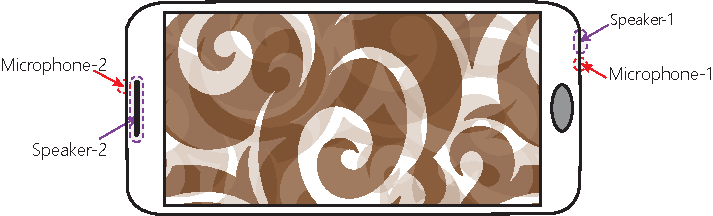
\includegraphics[width=0.7\textwidth]{figure/smartphone.pdf}
  \bicaption
    {智能手机上的音频设备}
    {Audio devices on smartphones}
  \label{fig:audio-device-smartphone}
\end{figure}

三星Galaxy S6是三星公司在2015年5月推出的一款智能手机,是本文原型系统ASSV使用的智能手机,因此以此为例进行说明。如图~\ref{fig:audio-device-smartphone}所示,该智能手机搭载了2个扬声器和2个麦克风:
\begin{enumerate*}[label=\alph*)]
    \item 一个降噪麦克风(Microphone-2)位于机身的上壁,对高频信号较为敏感,且原来用户打电话的时的发生点,可以用于记录背景噪声;
    \item 一个主麦克风(Microphone-1)位于机身的下壁,对人声比较敏感(通常低于8 kHz),用于记录通话语音;
    \item 一个通话扬声器(Speaker-2)位于屏幕上部,用于通话是对准耳朵;
    \item 一个主扬声器(Speaker-1)位于机身的下壁,位于主麦克风的旁边。
\end{enumerate*}

\begin{table}[!hpb]
  \centering
  \bicaption{三星Galaxy S6的硬件配置}{Hardware settings of Samsung Galaxy S6}
  \label{tab:smartphone-hardware-setting}
  \resizebox{\textwidth}{!}{
\begin{tabular}{|l|l|l|}
\hline
\multirow{2}{*}{Body}     & Dimensions  & 143.4 x 70.5 x 6.8 mm (5.65 x 2.78 x 0.27 in)                          \\ \cline{2-3} 
                          & Weight      & 138 g (4.87 oz)                                                                            \\ \hline
\multirow{4}{*}{Platform} & OS          & Android 5.0.2 (Lollipop), upgradable to Android 8.0 (Oreo); TouchWiz UI \\ \cline{2-3} 
                          & Chipset     & Exynos 7420 Octa (14 nm)                                                \\ \cline{2-3} 
                          & CPU         & Octa-core (4x2.1 GHz Cortex-A57 \& 4x1.5 GHz Cortex-A53)                \\ \cline{2-3} 
                          & GPU         & Mali-T760MP8                                                            \\ \hline
\multirow{2}{*}{MEMORY}   & Card slot   & No                                                                      \\ \cline{2-3} 
                          & Internal    & 32/64/128 GB, 3 GB RAM                                                  \\ \hline
\multirow{4}{*}{Sound}    & Loudspeaker & Yes                                                                     \\ \cline{2-3} 
                          & 3.5mm jack  & Yes                                                                     \\ \cline{2-3} 
                          &             & 24-bit/192kHz audio                                                     \\ \cline{2-3} 
                          &             & Active noise cancellation with dedicated mic                            \\ \hline
\multirow{5}{*}{Battery}  &             & Non-removable Li-Ion 2550 mAh battery                                   \\ \cline{2-3} 
                          & Charging    & Fast battery charging 15W                                               \\ \cline{2-3} 
                          &             & Qi/PMA wireless charging (market dependent)                             \\ \cline{2-3} 
                          & Talk Time   & Up to 17 h (3G)                                                         \\ \cline{2-3} 
                          & Music play  & Up to 49 h                                                              \\ \hline
\end{tabular}
}
\end{table}
该型号智能手机的硬件配置如表~\ref{tab:smartphone-hardware-setting}~\footnote{https://www.gsmarena.com/samsung\_galaxy\_s6-6849.php}所示,其具有较好的计算性能和较大的内存空间,支持24-bit/192kHz的音频设备,可以满足我们的对设备的要求。值得注意的是,从CPU型号上可得知,内存存储模式为小端模式,数据的低字节保存在内存的低地址。

\subsection{声波信号下转化}
\begin{figure}[!htp]
  \centering
  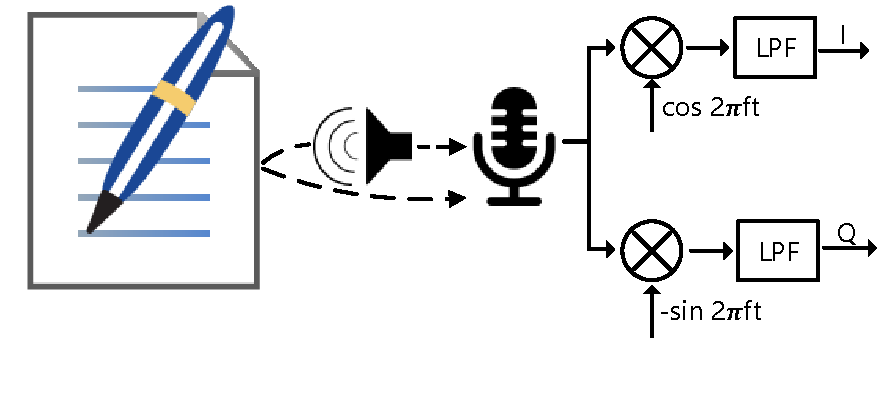
\includegraphics[width=0.7\textwidth]{figure/down-conversion.pdf}
  \bicaption
    {声波信号下转化}
    {Sound signal down conversion}
  \label{fig:sound-signal-down-conversion}
\end{figure}
假设智能手机上的麦克风的采样率设置为48 kHz。由于接收和发射声波的设备在同一智能手机,共享一个时钟频率,因此接收端和发送端之间不存在载频偏移(Carrier Frequency Offset, CFO)。因此,使用图~\ref{fig:sound-signal-down-conversion}所示的传统的相干解调器结构将所接收到的声波信号下转化为基带信号~\cite{tse2005fundamentals}。接收信号被分成两份副本,分别乘以发射信号$-cos2\pi ft$和它的相位偏移信号$-sin2\pi ft$,再经过一个低通滤波器获得同相(In-phase)和正交(Quadrature)分量。

LLAP~\cite{wang2016device}中对信号下转化的过程进行了解释。为了更好得理解数字下转化过程,我们假设一个信号路径$p$的路径长度随时间变化的函数为$d_p\left( t\right)$。来自信号路径$p$可以表示为:
$$
R_{p}\left( t\right) = 2A^{'}_{p}cos \left( 2\pi ft - 2\pi fd_{p}\left( t \right) / c - \theta_{p} \right),
$$
其中,$2A^{'}_{p}$是接收信号的强度,$2\pi fd_{p}\left( t \right)/c$是产生于传播延迟$\tau=d_{p}\left(t\right)/c$的相位间隔,$c$是声音传播速度。初始相位$\theta_p$是硬件延迟和由于反射而发生相位反转的结果。按照图~\ref{fig:sound-signal-down-conversion}中的结构,我们将接收信号乘以$cos\left( 2\pi ft \right)$,得到:
\begin{equation}\nonumber
\begin{aligned}
&2A_{p}^{'}cos \left( 2\pi ft - 2\pi fd_{p}\left( t\right)/c - \theta_{p} \right) \times cos\left( 2\pi ft\right) \\ 
= \quad &A_{p}^{'}\left( cos\left( -2\pi fd_{p}\left( t\right)/c - \theta_{p} \right) + cos\left( 4\pi ft - 2\pi fd_{p}\left( t\right)/c - \theta_{p} \right)  \right).
\end{aligned}
\end{equation}
第二个子项的频率为$2f$,属于高频,可以被低通滤波器所去除。所以我们可以获得基带信号的同相分量(I-component)为:
$$
I_{p}\left( t\right) = A_{p}^{'}cos \left( -2\pi fd_{p}\left( t\right)/c - \theta_{p} \right).
$$
相似地,我们可以获得正交分量(Q-component)为:
$$
Q_{p}\left( t\right)=A_{p}^{'}sin\left( -2\pi fd_{p}\left(t \right)/c - \theta_{p} \right).
$$
结合这两个分量,分别作为复数的实部和虚部,我们可以得到复数形式的基带信号($j^2=-1$):
$$
B_{p}\left( t\right) = A_{p}^{'}e^{-j\left( 2\pi fd_{p}\left( t\right)/c + \theta_{p} \right)}.
$$
因此,在路径$p$上的相位为:
$$
\phi_{p}\left( t\right) = -\left( 2\pi fd_{p}\left( t\right)/c + \theta_{p} \right),
$$当$d_{p}\left(t\right)$变化一个声波波长的长度$\lambda = c/f$时,相位$\phi_{p}\left( t\right)$变化$2\pi$。
\subsection{离散余弦变换}
DCT~\cite{ahmed1974discrete}是一种正交变换,可以用于实现一个维纳滤波器和模式识别中的特征选择。正交变换和逆变换在维纳滤波器中充当重要角色。在模式识别中,DCT可以用于特征选择,对原始数据进行降维,以便于进行分类。一个序列$X(m),m=0,1,\cdots,(M-1)$的DCT可以为定义为:
\begin{equation}
\label{equ:dct}
\begin{aligned}
G_{x}\left( 0\right) &= \frac{\sqrt{2}}{M} \sum_{m=0}^{M-1}X\left( m\right), \\
G_{x}\left( k\right) &= \frac{2}{M} \sum_{m=0}^{M-1}X\left( m\right)cos\frac{\left(2m+1\right)k\pi}{2M}, k=1,2,\cdots,(M-1).
\end{aligned}
\end{equation}
$G_{x}(k)$是第k个DCT系数。值得注意的是,基向量集合$\{ 1/\sqrt{2}, cos((2m+1)k\pi)/(2M) \}$实际上是一组离线切比雪夫多项式。
DCT的逆变换(Inverse Discrete Consine Transform, IDCT)可以被定义为:
\begin{equation}
\label{equ:idct}
X(m) = \frac{1}{\sqrt{2}}G_{x}(0) + \sum_{k=1}^{M-1}G_{x}(k)cos\frac{(2m+1)k\pi}{2M}, m=0,1,\cdots,(M-1). 
\end{equation}
在性能上,DCT好于离散傅里叶变换,接近于最优的Karhunen-Loeve Transform (KLT)。DCT的算法最简单的可以根据上诉的公式进行计算,原文\cite{ahmed1974discrete}中提出了可以使用快速傅里叶变换进行高效计算,之后研究者们提出了一些高效算法~\cite{winograd1978computing,lee1984new,hou1987fast}。

\subsection{卷积神经网络}
\begin{figure}[!htp]
  \centering
  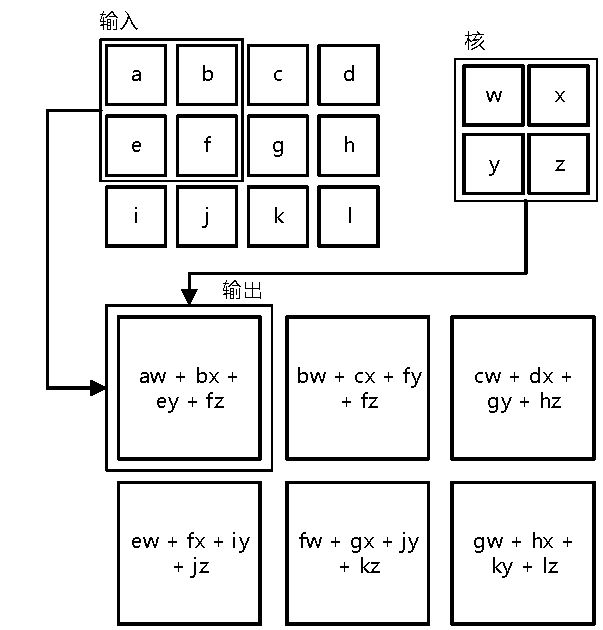
\includegraphics[width=0.4\textwidth]{figure/convolution-process.pdf}
  \bicaption
    {卷积过程}
    {Convolution process}
  \label{fig:convolution-process}
\end{figure}
CNN~\cite{goodfellow2016deep}是一种用于处理网格状数据的特殊ANN,通常包括两类操作:卷积和池化操作,在图像处理领域得到广泛应用。通常被实现为交叉相关函数的卷积操作,在一个输入2维图像(也可以是更高纬的张量)和一个卷积核上生成一个如下的特征图:
$$
S(i,j)=(K\times I)(i,j)=\sum_{m}\sum_{n}I(i+m,j+n)K(m,n),
$$
其中,$I$、$K$、$S$分别是输入图像、卷积核和特征图。图~\ref{fig:convolution-process}演示了一个在二维张量上的卷积运算过程。稀疏交互、参数共享和等变表示是卷积运算中的三个思想,三个思想之间互相影响,是的卷积神经网络只需要较少的模型参数便能实现可靠地特征提取。池化函数使用某个位置的相邻输出的总体统计特征来代替网络在该位置的输出,可对输入进行降维,为神经网络在提供了某种程度平移不变性,常用的池化函数有:最大池化函数、平均池化函数等。


\section{本章小结}
本章是手写签名认证相关技术的分析,首先分别从手写签名认证中的感知技术和手写签名认证中的建模方法两个方面对现有的研究进行了综述,然后分析总结了现有研究存在的问题。基于存在的问题,提出了本文的技术路线,最后介绍了本文中所涉及到的相关理论和技术。

\chapter{基于声波的签名认证方案的关键技术研究}
\section{问题描述与方案设计}
\subsection{问题描述}
本文要解决的问题是利用声波的相位相关信息实现手写签名认证,提出了一种基于声波的一个非侵入式、用户友好、安全、低延迟、准确的在线签名认证方案。其中需要考虑的几个关键的技术问题是音频设备硬件补偿技术技术问题、基于声波的相位相关信息的感知技术问题、基于声波的相位相关信息的特征提取技术问题、以及基于声波特征的建模技术问题。为解决上述问题,本文基于智能手机产品设计实现了一个手写签名认证系统,并在实际场景下部署测试了该系统。

本文列举两个签名认证的例子来描述应用场景,场景一描述我们生活中在银行柜台取款的常见场景便于理解手写签名认证系统的实际作用,场景二则描述了本文所设计系统的可应用场景:
\begin{enumerate}[label=(\arabic*)]
\item \textbf{场景一:}一位叫波波的小伙子去银行取存款,并申明他是这个存款账户的拥有者,然后银行职员要求他前面一边进行一下步操作。根据银行的实际情况,小伙子可能会在一张普通的纸上签字也可能在一个手写平板上签字。接着手写签名认证系统如下运行:首先它从数据库从查询了之前该小伙子留下的参考签名;下一步,它使用设定的算法比较查询签名和参考签名,并计算出查询签名和参考签名之间的相似度。如果系统实时运行的话,银行职员按照签名认证系统的输出结果实行下一步操作。显然,对于基于普通纸张的签名,一个静态的图像将会从纸张上扫描所得,此时签名认证系统为离线签名认证系;然而,基于手写平板的签名,一个额外的时间信息通常被用于提交认证的进度,此时的签名认证系统为在线认证系统。

\begin{figure}[!htp]
  \centering
  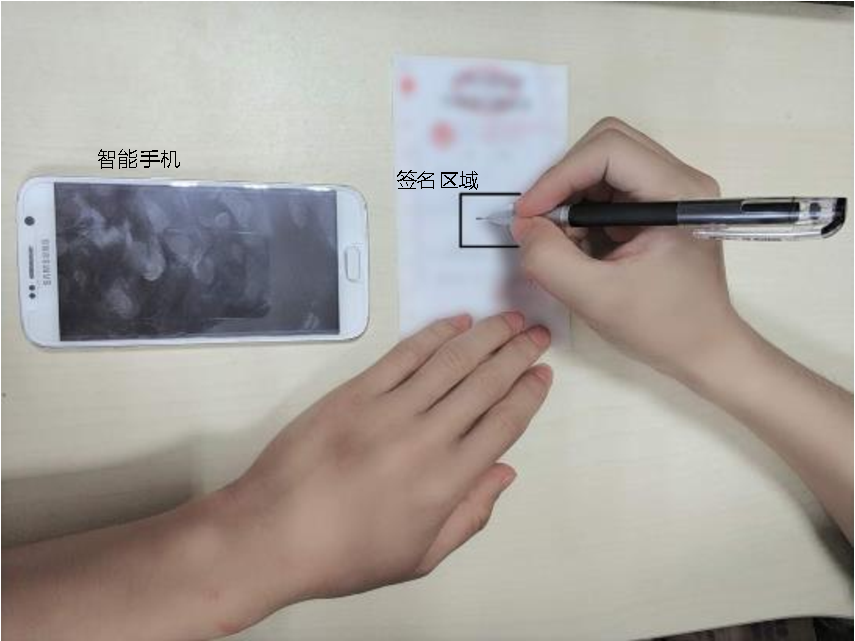
\includegraphics[width=0.6\textwidth]{figure/acoustic-senario.pdf}
  \bicaption
    {签名场景}
    {Senario of signing}
  \label{fig:sign-senario}
\end{figure}

\item  \textbf{场景二:}本文的签名认证方案可以作为一种需要和其他认证方案相结合的辅助认证方案,比如可以和现有的离线签证认证系统或者人工签名认证相集合,最终的系统利用多模的优势而提高签名认证精度。如图~\ref{fig:sign-senario}所示,当一个人在一张现金支票上的签名区域签名时候,他/她将他/她的智能手机放在签名区域旁边记录手和笔在签名动作过程中的模式,该模式将会发送去银行进行识别。纸上的签名将被扫描,作为离线签名认证系统的输入。同时使用不同的权重,两种签名认证方案可以得到融合。值得注意的是,可在支票打印一个二维码,通过二维码可以把智能手机获得签名模式和这个张支票联系起来。
\end{enumerate}

\begin{figure}[!htp]
  \centering
  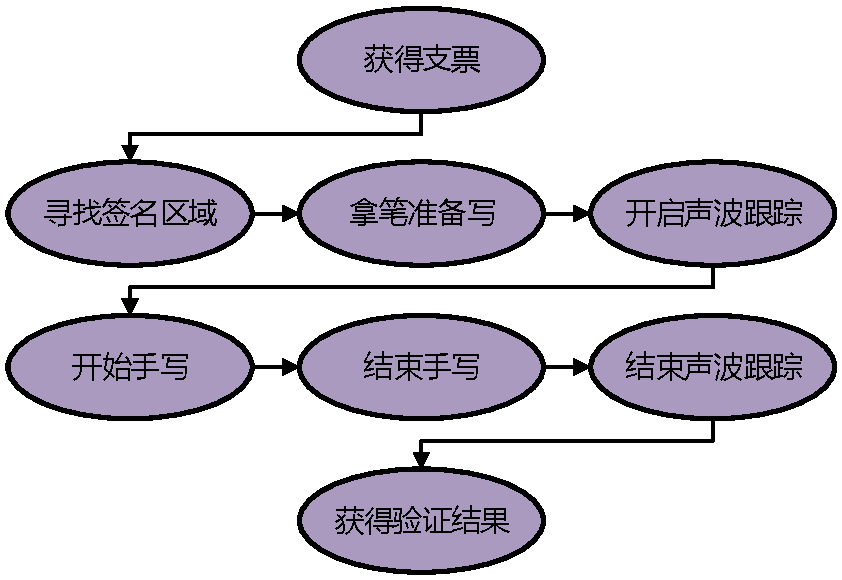
\includegraphics[width=0.6\textwidth]{figure/senario-actions}
  \bicaption
    {场景二签名步骤}
    {Signing steps in Senario 2}
  \label{fig:signing-steps}
\end{figure}

在两个场景中,我们默认认证参考签名已经预先被系统记录下。场景二本文系统所适用的场景,对签证者来说,他/她的操作包括:获取支票、寻找签名区域、拿笔准备写、开启声波跟踪、开始手写、结束手写、结束声波跟踪、获得验证结果。智能手机可以在场景中使用声波跟踪签名过程中手和笔的运动模式。虽然这个注意听起来十分鼓舞人心,但是使用智能手机收发声波跟踪手和笔运动实现在线认证的方案仍然面临着诸多挑战:首先,个人的签名仍然可以被观察和练习,这是目前所有签名认证系统所面临和需要克服的挑战;另外,声波可以被其他恶意的音频接收设备所接收,之后再播放出来实行重放攻击。

\subsection{方案设计}

\section{音频设备硬件补偿技术的研究}
\section{基于声波的相位相关信息的感知技术的研究}
\section{基于声波的相位相关信息的特征提取技术的研究}
\section{基于声波特征的建模技术的研究}
\section{本章小结}


\chapter{基于声波的签名认证方案的实验}
\section{实验准备}
\section{硬件补偿评估实验}
\section{精度评估实验}
\section{鲁棒性评估实验}
\section{微基准测试}
\section{经典系统对比实验}
\section{重放攻击实验}

\chapter{基于声波的签名认证方案的系统设计与实现}
\section{系统需求分析}
\section{系统设计与实现}
\section{系统性能评估}
\section{本章小结}

\chapter{总结与展望}
\section{工作总结}
\section{研究展望}
% \section{使用模板}

% \subsection{准备工作}
% \label{sec:requirements}

% 要使用这个模板撰写学位论文,需要在\emph{TeX系统}、\emph{TeX技能}上有所准备。

% \begin{itemize}[noitemsep,topsep=0pt,parsep=0pt,partopsep=0pt]
% 	\item {\TeX}系统:所使用的{\TeX}系统要支持 \XeTeX 引擎,且带有ctex 2.x宏包,以2017年或更新版本的\emph{完整}TeXLive、MacTeX发行版为佳。
% 	\item TeX技能:尽管提供了对模板的必要说明,但这不是一份“ \LaTeX 入门文档”。在使用前请先通读其他入门文档。
% 	\item 针对Windows用户的额外需求:学位论文模本分别使用git和GNUMake进行版本控制和构建,建议从Cygwin\footnote{\url{http://cygwin.com}}安装这两个工具。
% \end{itemize}

% \subsection{模板选项}
% \label{sec:thesisoption}

% sjtuthesis提供了一些常用选项,在thesis.tex在导入sjtuthesis模板类时,可以组合使用。
% 这些选项包括:

% \begin{itemize}[noitemsep,topsep=0pt,parsep=0pt,partopsep=0pt]
% 	\item 学位类型:bachelor(学位)、master(硕士)、doctor(博士),是必选项。
% 	\item 中文字体:fandol(Fandol 开源字体)、windows(Windows 系统下的中文字体)、mac(macOS 系统下的华文字体)、ubuntu(Ubuntu 系统下的文泉驿和文鼎字体)、adobe(Adobe 公司的中文字体)、founder(方正公司的中文字体),默认根据操作系统自动配置。
% 	\item 英文模版:使用english选项启用英文模版。
% 	\item 盲审选项:使用review选项后,论文作者、学号、导师姓名、致谢、发表论文和参与项目将被隐去。
% \end{itemize}

% \subsection{编译模板}
% \label{sec:process}

% 模板默认使用GNUMake构建,GNUMake将调用latemk工具自动完成模板多轮编译:

% \begin{lstlisting}[basicstyle=\small\ttfamily, caption={编译模板}, numbers=none]
% make clean thesis.pdf
% \end{lstlisting}

% 若需要生成包含“原创性声明扫描件”的学位论文文档,请将扫描件保存为statement.pdf,然后调用make生成submit.pdf。

% \begin{lstlisting}[basicstyle=\small\ttfamily, caption={生成用于提交的学位论文}, numbers=none]
% make clean submit.pdf
% \end{lstlisting}

% 编译失败时,可以尝试手动逐次编译,定位故障。

% \begin{lstlisting}[basicstyle=\small\ttfamily, caption={手动逐次编译}, numbers=none]
% xelatex -no-pdf thesis
% biber --debug thesis
% xelatex thesis
% xelatex thesis
% \end{lstlisting}

% \subsection{模板文件布局}
% \label{sec:layout}

% \begin{lstlisting}[basicstyle=\small\ttfamily,caption={模板文件布局},label=layout,float,numbers=none]
% ├── LICENSE
% ├── Makefile
% ├── README.md
% ├── bib
% │   ├── chap1.bib
% │   └── chap2.bib
% ├── bst
% │   └── GBT7714-2005NLang.bst
% ├── figure
% │   ├── chap2
% │   │   ├── sjtulogo.eps
% │   │   ├── sjtulogo.jpg
% │   │   ├── sjtulogo.pdf
% │   │   └── sjtulogo.png
% │   └── sjtubanner.png
% ├── sjtuthesis.cfg
% ├── sjtuthesis.cls
% ├── statement.pdf
% ├── submit.pdf
% ├── tex
% │   ├── abstract.tex
% │   ├── ack.tex
% │   ├── app_cjk.tex
% │   ├── app_eq.tex
% │   ├── app_log.tex
% │   ├── chapter01.tex
% │   ├── chapter02.tex
% │   ├── chapter03.tex
% │   ├── conclusion.tex
% │   ├── id.tex
% │   ├── patents.tex
% │   ├── projects.tex
% │   ├── pub.tex
% │   └── symbol.tex
% └── thesis.tex
% \end{lstlisting}

% 本节介绍学位论文模板中木要文件和目录的功能。

% \subsubsection{格式控制文件}
% \label{sec:format}

% 格式控制文件控制着论文的表现形式,包括sjtuthesis.cfg和sjtuthesis.cls。
% 其中,“cls”控制论文主体格式,“cfg”为配置文件。

% \subsubsection{主控文件thesis.tex}
% \label{sec:thesistex}

% 主控文件thesis.tex的作用就是将你分散在多个文件中的内容“整合”成一篇完整的论文。
% 使用这个模板撰写学位论文时,你的学位论文内容和素材会被“拆散”到各个文件中:
% 譬如各章正文、各个附录、各章参考文献等等。
% 在thesis.tex中通过“include”命令将论文的各个部分包含进来,从而形成一篇结构完成的论文。
% 对模板定制时引入的宏包,建议放在导言区。

% \subsubsection{各章源文件tex}
% \label{sec:thesisbody}

% 这一部分是论文的主体,是以“章”为单位划分的,包括:

% \begin{itemize}[noitemsep,topsep=0pt,parsep=0pt,partopsep=0pt]
% 	\item 中英文摘要(abstract.tex)。前言(frontmatter)的其他部分,中英文封面、原创性声明、授权信息在sjtuthesis.cls中定义,不单独分离为tex文件。
% 不单独弄成文件。
% 	\item 正文(mainmatter)——学位论文正文的各章内容,源文件是chapter\emph{xxx}.tex。
% 	\item 附录(app\emph{xx}.tex)、致谢(ack.tex)、攻读学位论文期间发表的学术论文目录(pub.tex)、个人简历(resume.tex)组成正文后的部分(backmatter)。
% 参考文献列表由bibtex插入,不作为一个单独的文件。
% \end{itemize}

% \subsubsection{图片文件夹figure}
% \label{sec:fig}

% figure文件夹放置了需要插入文档中的图片文件(支持PNG/JPG/PDF/EPS格式的图片),可以在按照章节划分子目录。
% 模板文件中使用\verb|\graphicspath|命令定义了图片存储的顶层目录,在插入图片时,顶层目录名“figure”可省略。

% \subsubsection{参考文献数据库bib}
% \label{sec:bib}

% 目前参考文件数据库目录只存放一个参考文件数据库thesis.bib。
% 关于参考文献引用,可参考第\ref{chap:example}章中的例子。
